%% Incluindo os pacotes necessários
\documentclass{beamer}
\usepackage[utf8]{inputenc}
\usepackage[portuguese]{babel}
\graphicspath{{images/}}

\usepackage{hyperref}
%\hypersetup{
    %colorlinks=true,
    %linkcolor=white,
    %filecolor=magenta,      
    %urlcolor=cyan,
%}

%\usetheme{Madrid}
%\usetheme{Copenhagen}
\usetheme{Ilmenau}
%\usecolortheme{beaver}
%\usecolortheme{orchid}
\usecolortheme{default}


%\usepackage{titlesec}
%\usepackage{titling}
%\usepackage{enumitem}
%\usepackage{indentfirst}
%\usepackage{graphicx}
%\usepackage{fancyhdr}
%\usepackage{color}
%\usepackage{fancyhdr}
%\usepackage{colortbl}
%\usepackage{framed}

%% Definindo o Autor e o título
\author[Levi, Victor]{Levi Cícero Arcanjo  \and Victor Emanuel Almeida}
\title{Apresentação - Projeto Sistemas Operacionais}
\date{Outubro - 2020}


\begin{document}
	\frame{\titlepage}
	\begin{frame}
		\frametitle{Conteúdo da apresentação}
		\tableofcontents
	\end{frame}
	
	
	\section{Item 2 do projeto}
	
	
\begin{frame}{Simulação dos algoritmos de escalonamento}
    \textbf{Características do programa:}
	\begin{itemize}
	    \item Linguagem: C++
		\item Algoritmos: 
		    \begin{itemize}
		        \item Round Robin
		        \item Shortest Job First
		    \end{itemize}
		 \item Todos os processos iniciaram juntos \\ (Possuem tempo de criação zero)
	\end{itemize}
\end{frame}

\begin{frame}{Simulação dos algoritmos de escalonamento}
    \textbf{Dados do Process Control Block implementado:}
	%\begin{itemize}
	    %\item Imagem
	%\end{itemize}
	\begin{figure}[!htb]
		\centering
		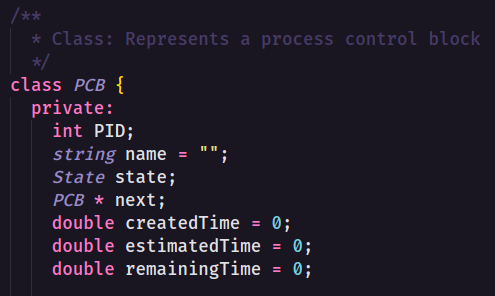
\includegraphics[keepaspectratio, scale=.6]{PCB.png}
		%\caption{\label{fig:PCB.png}Classe PCB}
	\end{figure}
\end{frame}

\begin{frame}{Algoritmos Utilizados}
    \textbf{Round Robin:}
	%\begin{itemize}
		%\item Definição: Algoritmo preemptivo que atribui fatias iguais de tempo a cada processo, manipulando todos os processos sem prioridade e em ordem circular.
		%\item Implementação: Imagem Aqui
	%\end{itemize}
	\begin{alertblock}{Definição}
Algoritmo preemptivo que atribui fatias iguais de tempo a cada processo, manipulando todos os processos sem prioridade e em ordem circular.
	\end{alertblock}
	\begin{figure}[!htb]
		\centering
		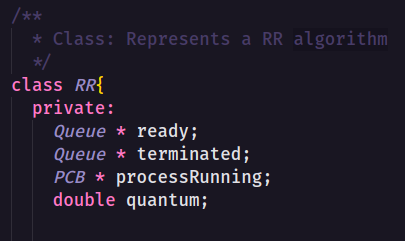
\includegraphics[keepaspectratio, scale=.6]{RR.png}
		%\caption{\label{fig:RR.png}}
	\end{figure}
\end{frame}

\begin{frame}{Algoritmos Utilizados}
    \textbf{Shortest Job First:}
	%\begin{itemize}
		%\item Definição: Algoritmo não preemptivo que seleciona para ser executado o processo com o menor tempo de execução.
		%\item Implementação: Imagem Aqui
	%\end{itemize}
	\begin{alertblock}{Definição}
		Algoritmo não preemptivo que seleciona para ser executado o processo com o menor tempo de execução.
	\end{alertblock}
	\begin{figure}[!htb]
		\centering
		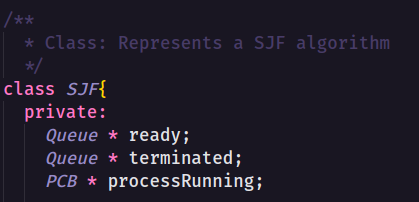
\includegraphics[keepaspectratio, scale=.6]{SJF.png}
		%\caption{\label{fig:SJF.png}}
	\end{figure}
\end{frame}

\section{Item 3 do projeto}
\begin{frame}{Problema clássico}
	\begin{itemize}
		\item Como problema clássico escolhemos o ``Leitores e escritores''
		\item Implementação com dois semáforos
		\item  \textcolor{cyan}{\href{https://github.com/arcanjolevi/projeto_1_so/blob/master/item_3/tabela.pdf}{Simulação do algoritmo}}
	\end{itemize}
\end{frame}

\section{Item 4 do projeto}
\begin{frame}{Código que utiliza a ideia de monitor}
	\begin{itemize}
	    \item Linguagem: Java
	    \item Implementação: Contador acessado por várias threads
	\end{itemize}
\end{frame}
\end{document}
